\chapter{Semantic similarity software suite} \label{chap:technical}

Working with Web Ontology language (OWL) files is not easy, especially when doing many small things a large number of times. Algorithms that depend on ontology information, such as semantic similarity, cannot be expected to load a set of potentially very large OWL files just to find specific facts represented therein, like what the superclasses of a given class are.

To satisfy the requirements of such algorithms, I propose a solution that enables programmatic access to the information contained in an ontology that does not depend on reading and parsing the ontology for every set of requests, but instead provides \emph{random access} to the elements of the ontology, including not only the concepts but also the axioms stated between them. The main idea of this solution is to insert \emph{useful} information from the OWL files into an SQL database, which can then be queried by semantic similarity algorithms. This software is called \owlsql.

Apart from this storage mechanism, I also produced and released a piece of software responsible for computing semantic similarity between concepts and annotated entities in a manner that
\begin{paralist}
    \item depends on the information stored by \owlsql, and
    \item uses a flexible model that can be quickly used by any developer to add their own semantic similarity algorithms.
\end{paralist}
This is called the Multi-Ontology Semantic Similarity (\mossy) tool.


\section{\owlsql} \label{sec:technical/owlsql}

\begin{note-paper}
    \owlsql's source code is available at \url{https://github.com/jotomicron/OWLtoSQL}.
\end{note-paper}

Biomedical ontologies are distancing themselves from the simple ``hierarchy of concepts'' model and are becoming increasingly more complex. As we saw in the previous chapters, ontologies contain disjointness information, existential quantifications, and even other types of axioms. For example, \ontology{FMA} contains the axiom
\begin{axiom}
    \existential{Heart}{has-part}{Aortic valve}
\end{axiom}
which means that for each \term{Heart}, there is some \term{Aortic valve} to which the heart is related by means of the property~\prop{has-part}; in less technical jargon, this means that all hearts have one aortic valve. Properties themselves are also related to each other, \eg \prop{negatively-regulates}, a property of \ontology{GO} that relates proteins with the processes that they inhibit, is a sub-property of \prop{regulates}.

On the one hand, this increased expressiveness leads to an increase in the richness of the information that can be represented in an ontology, ultimately allowing for a more faithful representation of the reality in a machine-understandable manner. On the other hand, this richness implies a certain complexity in the parsers of the language and an increased difficulty in extracting information from an OWL file in a \emph{random access} way. For example, finding the parts of the \term{Heart}, as represented in \ontology{FMA}, is a two-step task:
\begin{enumerate}
    \item \label{item:load-subtask} open and parse the \nolinkurl{fma.owl} file into RAM-accessible data structures; and
    \item query the data-structures for the necessary information.
\end{enumerate}

Several APIs (Application Programming Interfaces) have been created to perform these steps, such as Jena~\citep{Carroll2004} and OWL-API~\citep{Horridge2011}. Once opened, the extraction of information is mostly as a small sequence of look-up operations in RAM accessible hashmaps. However, for the one-time random access to the information, this solution is not suitable, as step~\ref{item:load-subtask} is time consuming and does not scale with the size of the ontology (to open and parse the aforementioned \nolinkurl{fma.owl} file, a regular-size personal desktop computer \mdash four 2GHz~CPUs and 4GB of RAM \mdash takes up to $30$~seconds). Having such a large waiting time for one semantic similarity request is highly undesirable: \eg a web service that computes semantic similarity between annotated entities and that takes $30$~seconds to return the similarity between \term{Heart} and \term{Trachea} will likely fail to be adopted by the community.

In order to solve this problem, there are two different possible avenues.

The first approach is to open the OWL file within a computer process capable of inter-process communication, which can then answer client questions like the one about the branches of the \term{Trachea}. This approach is quite flexible, since, given an appropriate protocol for the communication between server and clients, it allows the query of any OWL question. However, it is difficult to implement: the communication protocol between the processes needs to align with the OWL specification to ensure that all OWL-valid constructions can be queried and answered. While promising, this idea has yet failed to deliver fully functional software: the only existing implementation I know is OWLlink~\citep{Liebig2009}, which is still lacking some useful features. For example, it does not support asking for the names of the concepts, and it is not fully aligned with the latest OWL specification. Additionally, development has been stalled since August 2011.

The second approach is to open the OWL files and extract its information into a more accessible medium, such as a database. OWL can be fully serialised in RDF (see \secref{sec:concepts/semantic-web}), and as such RDF triple stores are an intuitive candidate for storing the OWL ontology, such as OpenRDF Sesame, Jena and OpenLink Virtuoso. These programs are, however, more suited for dealing with contexts where the ontology information is used to reason about the existing data, \eg to infer the type of some instances based on the properties asserted about those instance; instead, my work in semantic similarity is mostly related to querying the ontology itself: examples of question that are in realm of semantic similarity include ``what things are part of a \term{Heart}?''\ and ``what are the superclasses of \term{Aortic valve}?''. Additionally, querying over triple stores is usually done with SPARQL queries~\citep{Harris2013}, which is an OWL-agnostic language. While efforts have been made in order to introduce OWL-aware query languages, such as SPARQL-DL~\citep{Sirin2007} and SQWRL~\citep{OConnor2009}, they have not been implemented in any of the existing triple stores.

% As such, converting OWL requests into SPARQL queries requires an intimate knowledge of the RDF serialization of OWL: to query for the classes that are part of the ``Heart'' (\ie to find all \term{?x} such that \existential{Heart}{has-part}{?x}), one would need to use this corresponding SPARQL query:

% \begin{minted}{sparql}
% PREFIX rdfs: ???
% PREFIX owl: ???
% PREFIX fma: ???
% SELECT ?x WHERE {
%    fma:Heart rdfs:subClassOf ?y .
%    ?y a owl:Restriction ;
%       owl:onProperty fma:has-part ;
%       owl:someValuesFrom ?x .
% }\end{minted}

Furthermore, even a fully working triple store solution equipped with an OWL-aware query language can be slower than necessary for some user needs. For example, asking for all the leaf concepts (concepts which have no subclass of their own) may be a time consuming task, since it involves querying, for each concept, if it has any subclasses. While reasoners can alleviate this task by allowing certain queries to be performed faster (\eg reasoners build a static hierarchy that allows a quick answer to queries like ``Is $A$ a subclass of~$B$?''), some queries may still take a long time to run. In fact, a reasoner does not give the number of hypernymy relationships between two concepts, but only whether such a path exists. As such, it can be argued that some algorithms would benefit from a type of caching that computes a single time and stores the information they need in an easy-to-use, fast, and random-access back-end, which is not yet available.

In this context, it is relevant to introduce the idea of \emph{useful} information: presumably, an information-intensive algorithm such as semantic similarity has a static set of information requirements, an \emph{a-priori} established set of axiom types that are needed for the algorithm to work. For example, some semantic similarity algorithms need to know the superclasses of a given class and ``how far'' the superclass is to the class itself in the hierarchy. As such, and for the purpose of this discussion, I define \emph{useful} information as the total information that an algorithm needs to extract from the ontology in order to run without parsing the original OWL file and without performing time- and resource-consuming computations.

Based on this idea, I developed \owlsql, an extensible Java program that is responsible for reading OWL files using the OWL-API and saving any useful information into an underlying relational MySQL database. This allows random-access to any information that is encoded in the original ontology without the need to parse the ontology file again. Indices created on the stored tables guarantee fast retrieval of this information.

This is not the first time that a proposal like this has been made. \citet{Zhou2006} and \citet{Henss2009} proposed two previous solutions that tried to map all the OWL specification into a back-end database. These solutions, however, are buggy (I have in fact personally approached one of these authors requesting assistance with a bug I experienced, but their response was that they knew about the bug I was seeing, that it was due to a third party library, and that they could not offer further help), outdated (development has been stalled at least since 2010) and do not allow the insertion of non-standard information in the database (such as the edge distance in the class-subclass hierarchy). As such, I had to roll out my own solution.

Other papers have explored the idea of using OWL to build SQL databases, but they use OWL as a means to develop the database \emph{schema}, not to populate a database with the information encoded in the ontology \citep[\eg][]{Astrova2007,Zina2014}.


\subsection{The software model} \label{sub:owlsql/model}

From the point of view of its user, the interface of \owlsql\ is a configuration file that provides:
\begin{itemize}
    \item the settings needed to connect to the MySQL database;
    \item the list of ontologies that are to be loaded in memory and whose information is to be stored in the database; and
    \item a list of \emph{extractors}, which are Java classes that are responsible for extracting the information from the memory-accessible data-structures containing the ontologies and putting that information in the database.
\end{itemize}

\owlsql\ then
\begin{paralist}
    \item opens a connection to the MySQL server,
    \item loads the ontologies using OWL-API, and
    \item \emph{blindly} executes the code of each specified extractor.
\end{paralist}
Each extractor is an implementation of the abstract Java class \texttt{Extractor}, which provides convenience methods to access the MySQL database and the configuration options. In this manner, the definition of \emph{useful} information is provided by the user as the set of extractors to run (see \figref{fig:model}).

Importantly to the idea behind \owlsql\ is the notion that it is highly extensible. Anyone with knowledge of Java and the OWL-API can create their own Java class that extends \texttt{Extractor} and then use it as a \emph{plugin} to \owlsql.

\begin{figure}
    \centering
    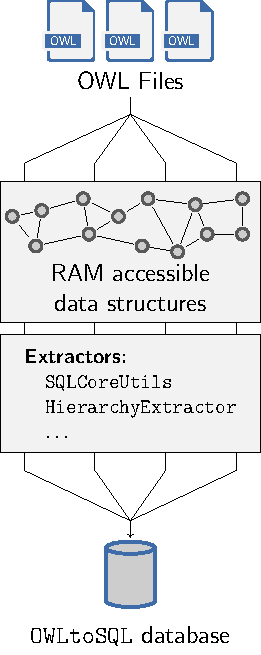
\includegraphics{images/owlsql.pdf}
    \caption[Operation model of \owlsql]{Several OWL files can be used by this software, which opens and parses them into memory-accessible data-structures (usually hashmaps that allow quick data lookup). Several Java classes extending a common interface named \texttt{Extractor} are then used to extract information from these data-structures and store it in the underlying database.}
    \label{fig:model}
\end{figure}


\subsection{Configuration file} \label{sub:owlsql/config}

\owlsql\ reads from a configuration file that the user is responsible for generating, which enables the user to choose the ontologies to load and extractors to run. The configuration file is written using JSON format and it must contain the following elements:
\begin{itemize}
    \item \json{mysql} determines the host, database name, user name and password needed to connect to the SQL server.
    
    \item \json{ontologies} is a list of strings, each containing the \texttt{url} that determines where the ontology should be loaded from. These options expect valid URLs that can be used by the OWL-API: as such, URL schemas such as \texttt{file:} or \texttt{http:} are supported.
    
    \item \json{extractors} contains a list of extractor specifications. These are themselves JSON objects containing a \json{class} element that points to the binary name of an extractor Java class and any additional elements that are used to tune the extractor's behaviour. In the case illustrated in \lstref{lst:owlsql-config}, the parameter \json{properties} contains the standard label property defined by the W3C committee~\citep{Guha2014}. Interpreting these options is the responsibility of the extractor class.
\end{itemize}

\begin{listing}
\centering
\begin{minted}{json}
{
    "ontologies": [
        "http://purl.obolibrary.org/obo/go.owl"
    ],
    "mysql": {
        "hostname": "localhost",
        "database": "db_name",
        "username": "user",
        "password": "passwd"
    },
    "extractors": [
        {
            "class": "pt.owlsql.extractors.NamesExtractor",
            "properties": [
                "http://www.w3.org/2000/01/rdf-schema#label"
            ]
        },
        {
            "class": "pt.owlsql.extractors.HierarchyExtractor",
        },
        {
            "class": "pt.owlsql.extractors.LeavesExtractor",
        }
    ]
}
\end{minted}
\caption[A possible \owlsql\ configuration file]{These examples shows the configuration that needs to be provided to \owlsql\ in order to store the information represented in the Gene Ontology, and specifies that the information to extract is the labels of the concepts, the class-subclass hierarchy and the set of leaf concepts.}
\label{lst:owlsql-config}
\end{listing}

More than one extractor can be given (as exemplified in \lstref{lst:owlsql-config}), and the order in which they are given in the configuration file is the order in which they are executed by \owlsql.


\subsection{Built-in extractors} \label{sub:owlsql/builtin}

Even though \owlsql\ provides the possibility for user-defined extractors, it provides a significant number of built-in extractors. I mention five of them, as an illustration.

The most important one, which is fundamental for the proper functioning of this software, is named \texttt{SQLCoreUtils} and it is responsible for extracting the bare minimum information from the OWL files: the entities represented in each loaded ontology. Each entity is stored in a master table and a unique integer identifier is provided to it. This identifier is more suitable for database management than the actual Internationalized Resource Identifier (IRI) (see \secref{sec:concepts/owl}) that ontologies provide, as integers can be more easily indexed than the IRI of the entities, which are text that is, in principle, not bounded by a maximum length. The table saves the identifier, the IRI of the entity, and the type of OWL entity that it represents. For example, if an ontology makes use of the concept \nolinkurl{http://www.w3.org/2002/07/owl\#Thing}, this entity is stored in the database as an \texttt{OWLClass} associated with that IRI, and a unique integer identifier is assigned to it.

\texttt{HierarchyExtractor} builds and stores the full class-subclass hierarchy of the loaded ontologies. Take for instance the small ontology illustrated in \figref{fig:small-ontology}; this extractor stores in the database the facts ``\term{Wolf} \prop{is-a} \term{Mammal}'' and ``\term{Cow} \prop{is-a} \term{Mammal}'', which are direct class-subclass relationships, but also facts like ``\term{Wolf} \prop{is-an} \term{Animal}'', which can only be obtained by traversing two relationships. As such, along with each fact, this extractor stores the minimum distance between the two classes.

\begin{figure}
    \centering
    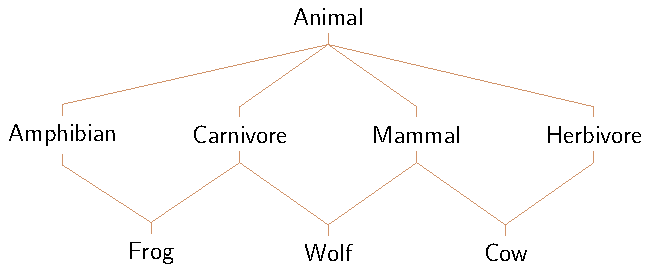
\includegraphics{images/animal-ontology.pdf}
    \caption[A toy ontology representing some animals]{The classes are organised in a class-subclass hierarchy, where the maximum distance between any concept and the root is $2$.}
    \label{fig:small-ontology}
\end{figure}

\texttt{LeavesExtractor} creates a table that contains the leaves of the ontologies, \ie the classes that have no subclass. This extractor depends on the information stored by the previous one, and as such must always be executed after the previous one.

\texttt{ICExtractor} calculates the information content of each concept (see \secref{sec:sota/node}, specifically \eqref{eq:resnik-ic,eq:seco}). Four different algorithms are calculated and stored in the database.

\texttt{NamesExtractor} stores the names of the concepts of the ontologies in the database. By default, this extractor uses the property \prop{rdfs:label} to find the names of entities, but it is possible to specify a different property in the configuration file (see~\lstref{lst:owlsql-config}).


\subsection{Retrieval from the database} \label{sub:owlsql/retrieval}

The retrieval of information from the database is done directly from the database. This requires that the users of the \owlsql\ back-end are familiar with how the information is stored in the database.

While there are some disadvantages to this (the information is stored in a non-standard format), proper documentation can mitigate these aspects. On the other hand, this allows any programming language that has a MySQL driver to access the information.

% For example, the \texttt{SQLCoreUtils} includes the following methods:
% \begin{itemize}
%   \item \texttt{getAllEntities()}: retrieves a set containing all the OWL entities stored in the database
  
%   \item \texttt{getDefiningOntologies()}: retrieves the \texttt{OWLOntologyID} of the ontologies that make use of a given OWL entity
  
%   \item \texttt{getEntity(int)}: retrieves the OWL entity that corresponds to the given internal ID. This method is essential for applications that need to retrieve information from the database, since the information is stored in terms of the internal Identifiers, but applications want the actual OWL entities.
  
%   \item \texttt{getID(OWLEntity)}: this is the reverse of the previous method; it returns the internal ID of a given OWL entity.
% \end{itemize}

% These methods are extensively used by the other extractors, particularly the \texttt{getID()} method. For example, \lstref{lst:hierarchy-snippet} shows a snippet of the extracting method of \texttt{HierarchyExtractor}. It uses the method \texttt{SQLCoreUtils.getID()} to convert the OWL classes into internal unique identifiers that are then inserted into the table (see lines~1, 15 and~16).

% \begin{listing}
% \centering
% \begin{minted}[gobble=4]{java}
%     SQLCoreUtils utils = getDependency(SQLCoreUtils.class);
    
%     PreparedStatement insertStatement = getConnection().prepareStatement(
%         "INSERT INTO hierarchy (subclass, superclass, distance) " +
%         "VALUES (?, ?, ?)");
    
%     insertStatement.setInt(3, 1); // Distance is 1 for direct class-subclass
%     for (OWLSubClassOfAxiom ax : ontology.getAxioms(AxiomType.SUBCLASS_OF)) {
%         OWLClassExpression subClass = ax.getSubClass();
%         OWLClassExpression superClass = ax.getSuperClass();
    
%         if (subClass.isAnonymous() || superClass.isAnonymous())
%             continue;
    
%         int subClassID = utils.getID(subClass.asOWLClass());
%         int superClassID = utils.getID(superClass.asOWLClass());
    
%         insertStatement.setInt(1, subClassID);
%         insertStatement.setInt(2, superClassID);
%         insertStatement.execute();
%     }
% \end{minted}
% \caption{A snippet of the \texttt{HierarchyExtractor} extractor, showing its usage of the \texttt{SQLCoreUtils} class.}
% \label{lst:hierarchy-snippet}
% \end{listing}

% Other extractors also provide retrieval mechanisms for the information that they have stored. For example, the \texttt{HierarchyExtractor} has a \texttt{getDepth(int)} method, which returns the maximum distance between a class and the root of the ontology. It also provides the \texttt{getSuperclasses(int)} (resp.~\texttt{getSubclasses(int)}) method, which take as input the database ID of an OWL class and returns the set of OWL classes that are superclasses (resp.~subclasses) of the input.

% The existence of these retrieval methods provides users with the ability to use \owlsql\ not only to save information in the database but also to retrieve it later, when needed, in an abstracted way that hides the details of the underlying database.


\subsection{Conclusions} \label{sub:owlsql/conclusion}

\owlsql\ converts OWL files into random-access information in a MySQL database, allowing researchers to streamline work flow that depends on the axioms provided by these files. It is configured with a JSON file that describes the type of information that is needed for downstream applications and provides a series of built-in extractors to actually convert OWL axioms into MySQL tables and rows. Furthermore, it is extensible, which means that Java programmers can create extractor classes that take care of information not already covered by the built-in extractors.

In this sense, I think \owlsql\ contributes to the current panorama in the web semantic by giving ontology users the power to more easily access the axioms they contain.

% \owlsql\ was a major undertaking from my part. I was originally interested in creating an application using the client-server model, where the server program reads the OWL files to memory and then several client programs would make OWL requests to the server (similar to how OWLlink is supposed to work~\citep{Liebig2009}). Unable to produce a satisfactory solution based on this idea, I ended up having to create \owlsql\ from scratch, invalidating all the previous work.


\newpage

\section{\mossy} \label{sec:technical/mossy}

\begin{note-paper}
    \mossy's source code is available at \url{https://github.com/jotomicron/MOSSy}.
\end{note-paper}

\owlsql\ stores OWL axioms and other pre-computed information in a database, providing random-access to it. This enables semantic similarity algorithms to exploit the knowledge stored in the database and, therefore, to more quickly perform their calculations. In this section, I present the Multiple-Ontology Semantic Similarity tool (\mossy), which implements semantic similarity measures precisely by leveraging on an \owlsql\ database. This dependence means that \mossy\ can quickly calculate ontology-based semantic similarity without having the need to wait for the long loading and parsing times associated with reading an OWL file.

Furthermore, by being an open-source tool that can be extended with more similarity algorithms, it can be regarded as a way to reproducibly compare ontology concepts and annotated entities, thus improving the general state of the art in this field of research.


\subsection{Software model} \label{sub:mossy/model}

\mossy\
\begin{paralist}
    \item connects to an \owlsql\ database,
    \item reads a configuration file to obtain the set of objects to compare and the semantic similarity algorithm to use,
    \item performs the comparisons, and
    \item outputs the resulting similarity values.
\end{paralist}
With this model in mind, \mossy\ is actually a thin wrapper around the semantic similarity algorithms. It is coded in Python rather than Java because, given Python's dynamic nature, algorithms can handle the similarity between two concepts or between two annotated entities. In a typed language like Java, achieving the same goal is cumbersome; in particular, the \mossy\ framework would only allow explicitly defined types of entities to be used, while Python allows all possible entity types to be used, due to its duck typing mechanism. On the other hand, Python is one of the languages of choice in bioinformatics, being known and used by $46\%$~of bioinformaticians, contrasting with the~$18\%$ that use Java (survey from 2012~\citep{Barton2012}).

The real power of \mossy, similarly to \owlsql, comes from the ability to quickly and easily implement new semantic similarity algorithms that depend on the data extracted by \owlsql. In fact, any Python class that implements a \texttt{compare} method that takes two arguments can be specified by the user to perform the comparison. See \secref{sub:mossy/extensibility} for an example. Additionally, the internal \mossy\ API contains convenience methods to access the database information, thus accelerating the process of implementing an algorithm even further.

Additionally, given Python's duck typing mechanism, the user can implement methods to compare not only concepts with other concepts, but any object, as long as the algorithm supports it. For example, we will see in the next section that \mossy\ can be used to compare lists of concepts with other lists of concepts, but nothing in the software model needs to be changed to accommodate for that difference, as there is no type requirements for the \texttt{compare} method.

Finally, the configuration file is similar to an actual Python script, where the user specifies the comparer and can provide it with parameters if necessary using a familiar syntax.


\subsection{Configuration parameters} \label{sub:mossy/config}

\mossy\ expects from the user a configuration file that contains the following information:
\begin{paralist}
    \item the database connection parameters (database, user name and password),
    \item the semantic similarity algorithm to apply, and
    \item the pairs of objects to compare.
\end{paralist}
An example of a configuration file is presented in \lstref{lst:mossy-config}. If \owlsql\ has been executed to extract the information from \ontology{GO} and \ontology{CHEBI}, this configuration file would produce the output presented in \lstref{lst:mossy-results}.

\begin{listing}
\centering
\begin{minted}[gobble=4]{python}
    database = "my_owlsql"
    username = "johndoe12"
    password = "mypasword"
    
    namespaces = {
        "GO": "http://purl.obolibrary.org/obo/GO_"
        "CHEBI": "http://purl.obolibrary.org/obo/GO_"
    }
    
    comparer = simple_model_comparer(
        inner=simgic(ic="seco"),
        aggr=model_avg())
    
    model1 = { "GO": ["GO:0005829", "GO:0008307", "GO:0030049"],
               "CHEBI": ["CHEBI:15377", "CHEBI:16788"] }
    model2 = { "GO": ["GO:0035252", "GO:0016266"],
               "CHEBI": ["CHEBI:23588", "CHEBI:15377"] }
    model3 = { "GO": ["GO:0035252"],
               "CHEBI": ["CHEBI:23588", "CHEBI:62777"] }

    pairs = [(model1, model2), (model1, model3), (model2, model3)]
\end{minted}
\caption[A possible \mossy\ configuration file]{From top to bottom, this configuration file defines
\begin{paralist}
    \item the database parameters (\texttt{database}, \texttt{username}, and \texttt{password}),
    \item two namespaces (so that the user can refer to concepts in a more succinct manner),
    \item the algorithm used to compare the entities (\texttt{comparer}), in this case a model comparer that uses $\sim[GIC]$ to compute similarity between lists of concepts and aggregates the values by taking their average,
    \item the objects being compared (\texttt{model1}, \texttt{model2} and \texttt{model3}), and
    \item the pairs that are to be compared, in this case all the possible pairs are present.
\end{paralist}}
\label{lst:mossy-config}
\end{listing}

\begin{listing}
\centering
\begin{minted}[gobble=4]{text}
    model1  model2  0.18541
    model1  model3  0.84711
    model2  model3  0.21003
\end{minted}
\caption[\mossy\ output]{This is the output that results from running \mossy\ using an underlying database containing the information on \ontology{GO} and \ontology{CHEBI}.}
\label{lst:mossy-results}
\end{listing}


\subsection{Built-in algorithms} \label{sub:mossy/builtin}

\mossy\ already contains several built-in semantic similarity measures, which I divide in three groups:

First, it contains algorithms to compare concepts with concepts. In this category, \mossy\ provides the measures proposed by \citet{Resnik1995}~(\eqref{eq:resnik-ssm}), \citet{Lin1998}~(\eqref{eq:lin}) and \citet{Jiang1997}~(\eqref{eq:jiang}). The user can provide parameters to these algorithms (see \secref{sub:mossy/config}) to specify which hierarchies to use in these measures (\eg \ontology{GO} semantic similarity measures can use a hierarchy containing both \prop{is-a} and \prop{part-of} relationships simultaneously~\citep{Lord2003}), and whether to include a disjointness factor, according to the description in \secref{sec:enhancements/disjointness}.

Second, it also has algorithms that deal with lists of concepts. On the one hand, it provides the $\sim[UI]$~(\eqref{eq:simui}) and $\sim[GIC]$~(\eqref{eq:simgic}) algorithms, which compare lists of concepts directly; on the other hand, it provides composable approaches that create a similarity matrix with a user-specified concept-to-concept algorithm and then aggregate the several values in the matrix into a single similarity result (see \figref{fig:bma}). In this last case, the user can specify exactly which concept-to-concept comparer they want to apply and which aggregation strategy to follow.

Finally, \mossy\ provides ``model comparison'' algorithms, which compare a model with another model. For the purpose of this software, a ``model'' is dictionary that associates a domain with a list of concepts. This notion is important when dealing with multiple domains: \eg when dealing with biomodels (see \secref{sec:data/biomodels}), it is relevant to use information on enzymes and on chemical compounds, which come from \ontology{GO} and \ontology{CHEBI} respectively. To compare such biomodels with one another it is important to be able to separate \ontology{GO} concepts from \ontology{CHEBI} concepts in different groups. To achieve this, \mossy\ expects a dictionary where each key is the name of a domain and the values are lists of terms from that domain (see an example in \secref{sub:mossy/config}). In this scenario, a model comparer will use internally a list comparer to compare the \ontology{GO} list of one biomodel to the \ontology{GO} list of the other model (likewise for the \ontology{CHEBI} lists) and aggregates the two values according to some user-specified mechanism, like the average, the maximum or the minimum.


\subsection{Extensibility} \label{sub:mossy/extensibility}

\mossy\ facilitates the implementation of new semantic similarity algorithms. The similarity developer needs only to make sure that the information that the algorithm needs to use has been successfully extracted to the underlying \owlsql\ database. For example, the code in \lstref{lst:mossy-plugin} implements an algorithm that returns the \emph{distance} (rather than similarity) between two terms in the class-subclass hierarchy.

\begin{listing}
\centering
\begin{minted}[gobble=4]{python}
    from mossy import sql, utils
    from mossy.parse_config import register
    
    @register()
    class edge_distance:
        def compare(self, one, two):
            one = utils.get_id(one)
            two = utils.get_id(two)
            
            sql.cursor.execute("""
                SELECT MIN(h1.distance + h2.distance)
                FROM hierarchy AS h1, hierarchy AS h2
                WHERE h1.subclass = %s AND h2.subclass = %s
                  AND h1.superclass = h2.superclass
            """, (one, two))
            
            return sql.cursor.fetchone()[0]
\end{minted}
\caption[The code of a new \mossy\ plugin]{This code effectively describes a comparer that calculates the distance between two concepts be counting the number of edges between them in the class-subclass hierarchy extracted to the underlying database.}
\label{lst:mossy-plugin}
\end{listing}

Saving this file in a directory that \mossy\ recognises is all it takes to enable the user to use the algorithm \texttt{edge\_distance} in their configuration file.


\subsection{Conclusion} \label{sub:mossy/conclusion}

\mossy\ provides a mechanism to allow quick implementation of semantic similarity measures based on OWL ontologies and on the OWL information that has been extracted to an underlying \owlsql\ database (it does not require loading and parsing OWL files because \owlsql\ takes care of producing a database where all the needed information is stored). Furthermore, it enables users to easily create a configuration file containing the pairs of objects that they want to compare and the algorithm that they want to use, producing a \texttt{TSV} file with the results of performing the comparison.

Finally, \mossy\ contributes to the current panorama in semantic similarity measures, providing a reproducible mechanism to deal with multiple ontologies. Its software model allows quick implementation of measures to be tested, but also allows its use in a production environment.

